\chapter{State of the Art}
\label{chap:sota}
% Motivation and definition

In this chapter, we will discuss the state of the art related to control of Boolean networks. We will start with a brief overview of the history of control theory and control of partially specified systems. We will then focus on control of synchronous, asynchronous and most-permissive BN which served as an inspiration of development of the \PBN{} control methods presented in the following chapters (\autoref{chapter:source_target_control} and \autoref{chapter:phenotype_control_psbn}). Next, we discuss overlap and applicability of control to the problematic of model inference. Finally, we exhaustively compare the existing control methods and tools in the field of BN control and discuss the limitations of the existing methods and tools.

\section{Control of discrete systems}
\marginpar{
    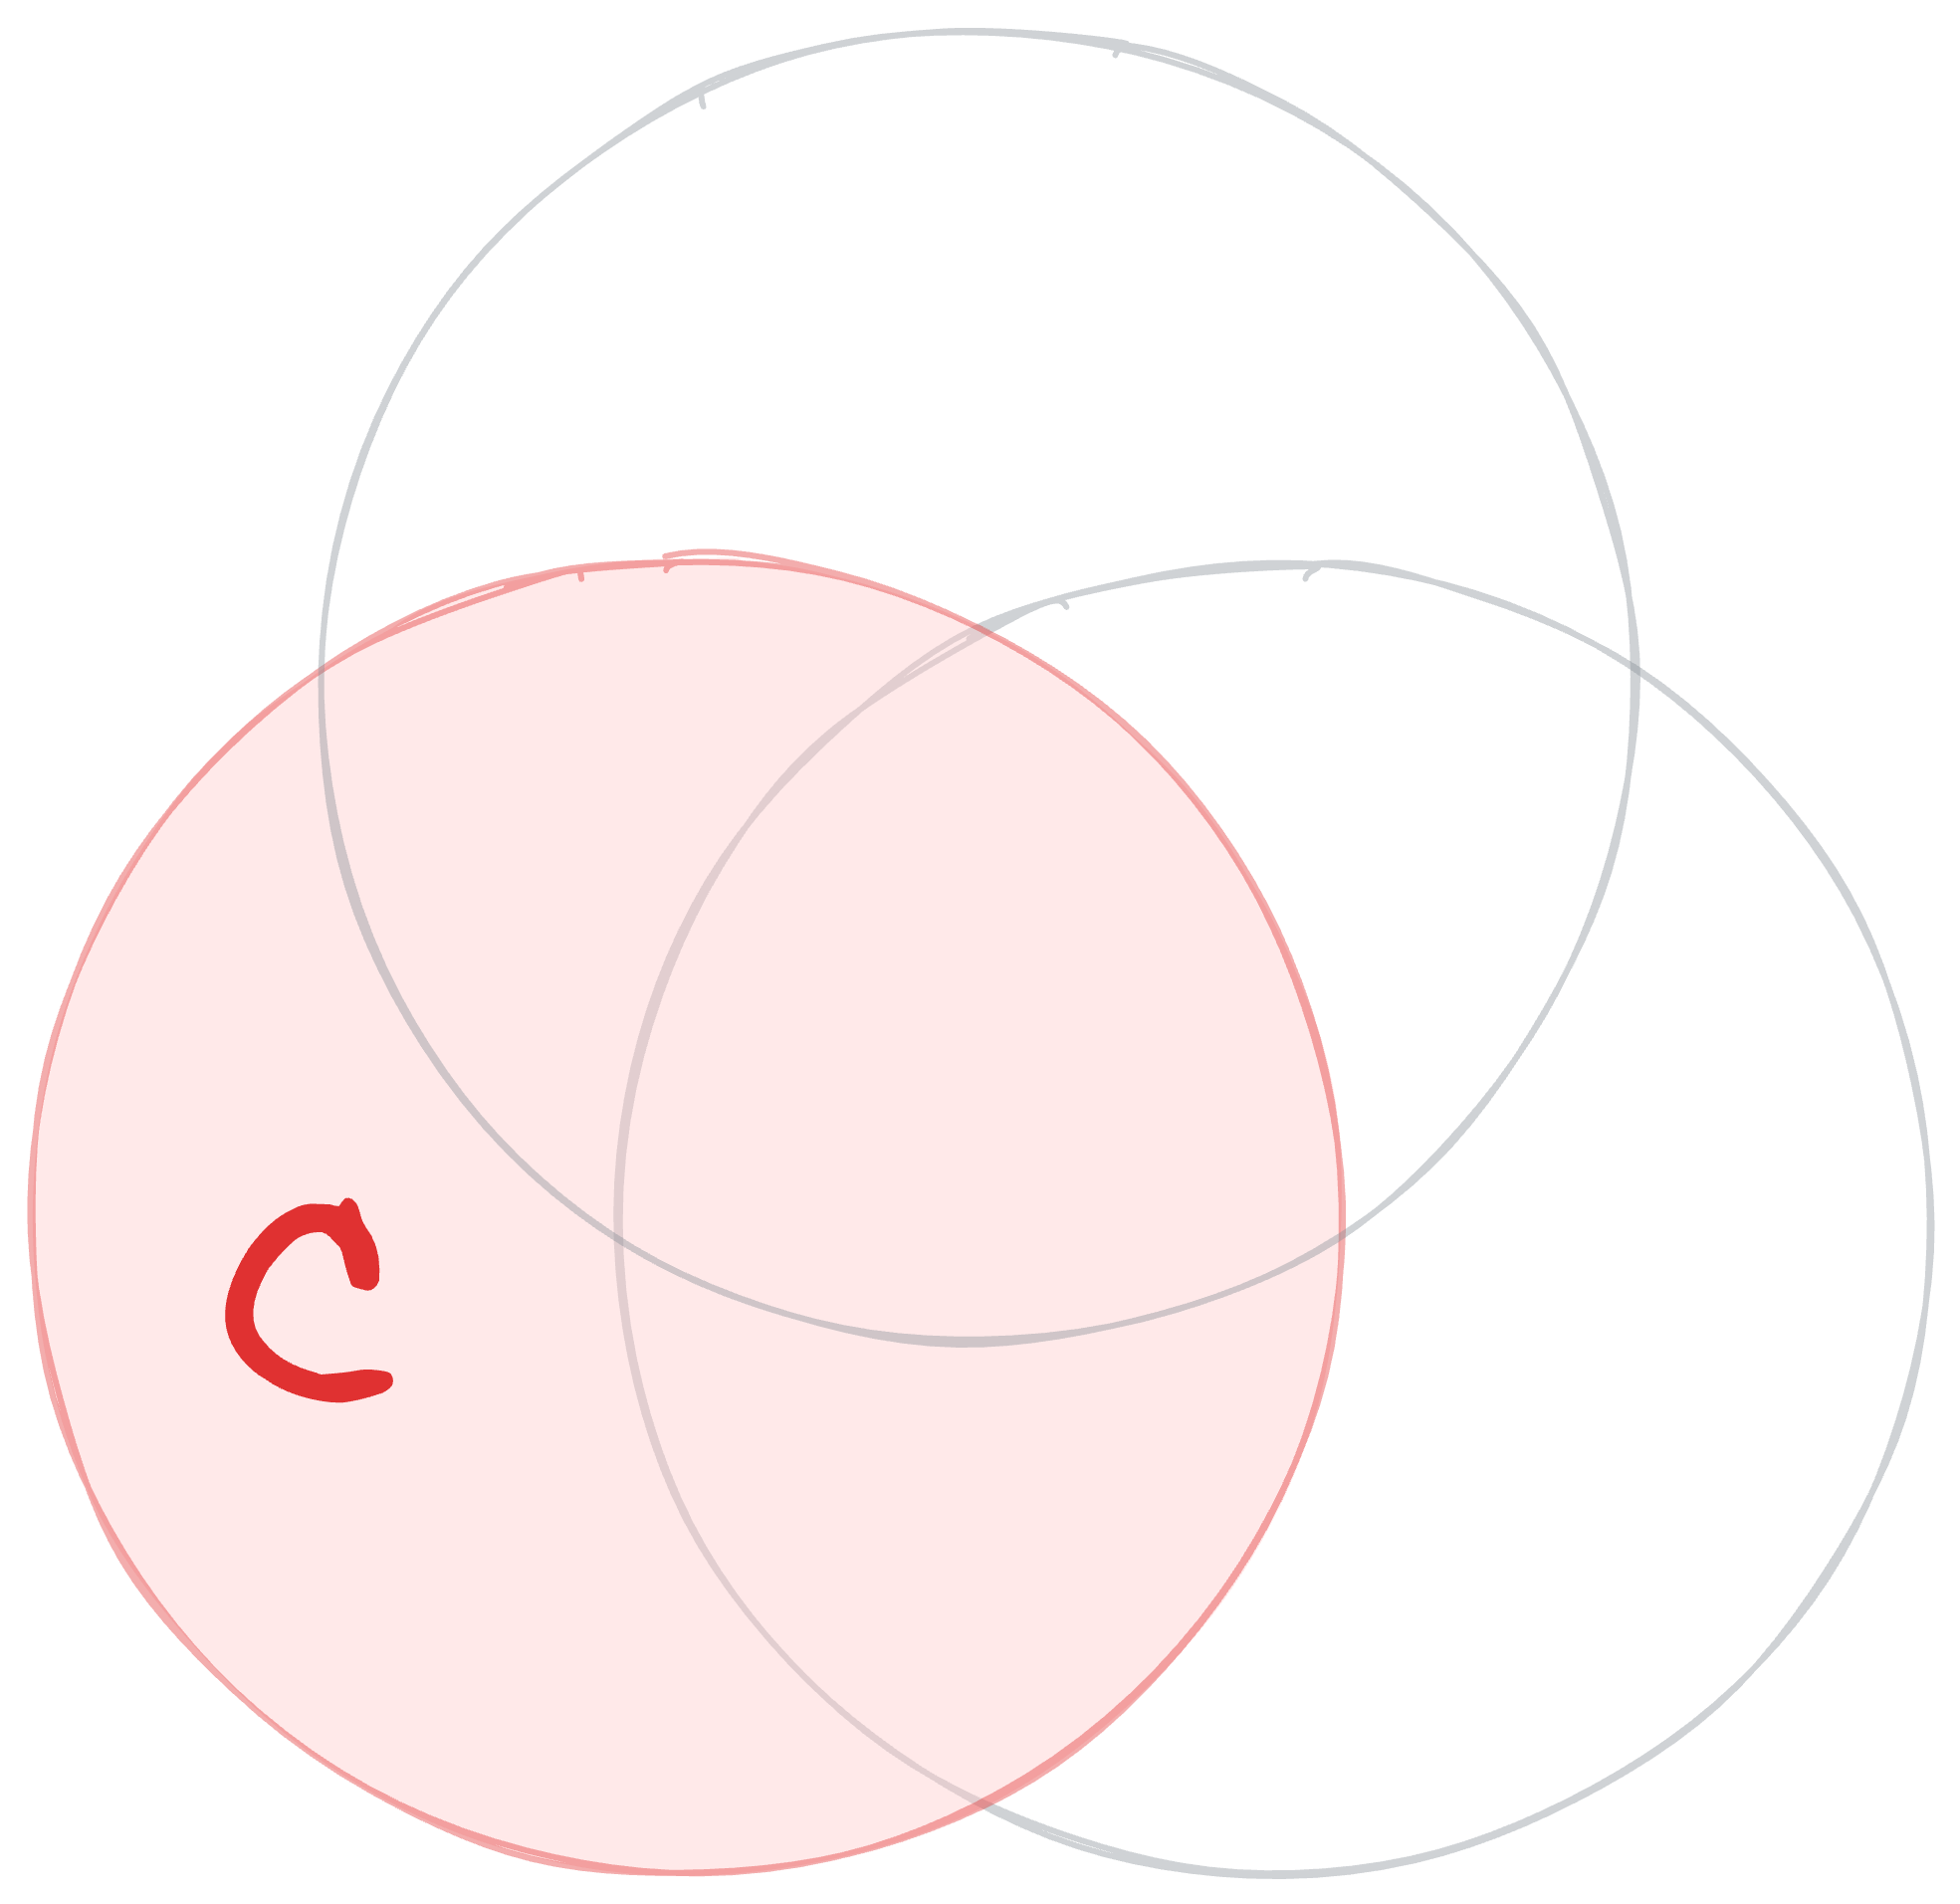
\includegraphics[width=\marginparwidth]{Figures/topics_ctrl.png}
}
\label{sec:controlDiscrete}

% History since Maxwell & slightly before
The field of control theory has an extensive historical background, tracing back to the 19th century when James Clerk Maxwell formalized the principles of feedback through his seminal work on governors~\cite{Maxwell1868}. These mechanical regulators, such as the centrifugal governor used to maintain windmill speed~\cite{Fernandez2003}, embodied some of the earliest notions of automatic control, though their application was predominantly focused on systems governed by continuous dynamics.

% First Discrete systems control -> relay circuits
As engineering advanced into the early 20th century, a paradigm shift towards discrete systems began with the rise of relay logic and switching circuits. Pioneered by Claude Shannon in his groundbreaking master's thesis~\cite{Shannon1938,Shannon1940}, the application of Boolean algebra to electrical circuits laid the foundation for the control of discrete systems. This marked the transition from purely continuous control to symbolic, state-based reasoning in control design.


% Cybernetics overarching
The 1940s brought a unifying conceptual breakthrough with the emergence of cybernetics. Led by Norbert Wiener, who was himself inspired by Maxwell’s early insights, cybernetics established a theoretical framework for feedback, communication, and control across mechanical, biological and combined systems~\cite{Wiener1948}. This new perspective helped shape the modern view of control as a universal system principle,  leading to its widespread application in fields such as engineering, economics, cognitive science, and biology.

% DES
From this foundation, the control of discrete systems evolved into more specialized subfields. One of the most prominent is the control of discrete event systems (DES), introduced by Ramadge and Wonham~\cite{Ramadge1987}. In DES, the processes under control are modeled as asynchronous, discrete, and potentially nondeterministic systems. These systems are often described by formal languages, where the plant is represented as a language generator and the controller (or supervisor) as a recognizer of a target language. The central problem becomes the synthesis of the largest controllable sub-language that satisfies the desired specifications

% Model checking? Thin ice :/ 
One of the major advancement in the discrete systems theory is the development of model checking~\cite{Clarke1981,Clarke1997}. Model checking is a formal verification method used to determine whether a system model (e.g. a Kripke structure~\cite{Kripke1959,Kripke1963}) satisfies a temporal logic specification (e.g. a LTL~\cite{Pnueli1977}). It has been instrumental in verifying properties such as safety, liveness, and reachability. A \emph{parametric} model checking or ~\emph{parameter synthesis} then seeks to find the maximal set of parameters for which the property holds~\cite{Hune2002,Daws2004,Smijakova2020}.

% Model checking -> less (parameter) options, more general properties
% Control -> very specific property types, more flexible parameters/perturbations/interventions
Formulas such as ensuring a system "eventually reaches a desired state" can be also viewed as a direct reduction of the control problem. This brings us to a provocative question -- what is the relationship between control and parametric model checking? The two problems share a common goal of refining system behavior to meet certain specifications, but they approach the problem from different angles. Model checking typically operates within a well-defined domain of parameters and verifies whether a selected property (drawn from a wide variety of types) holds for a given system. 

Control theory, on the other hand, tends to focus on a narrower set of property types (i.e., reachability) but allows for greater flexibility in choosing parameters, applying perturbations, or designing other interventions to guide system behavior. Specifically, parameter synthesis typically infers a static system properties, whereas control might also apply temporal interventions. Therefore, narrowing the focus to a specific property type enables more efficient optimization for the problem at hand.

% Booelan control networks
The control of discrete systems eventually extended to the realm of BN theory thoroughly introduced in the previous chapter. Initially, Boolean \emph{control} networks (BCN) were considered as an object of the control~\cite{Akutsu2007,Cheng2010,Hochma2013,Zhao2015,Moradi2019}. BCNs are characteristic by containing a set of control (input) nodes and a set of controlled (output) nodes. The control problem lies in the assigning Boolean values to the given control inputs. This problem was extensively studied and successfully solved e.g. using algebraic and semi-tensor product methods~\cite{Cheng2010} or model checking~\cite{Langmead2009}. 

It could be argued, that BCN control problem is more similar to the flavor of parameter synthesis, than to the control of discrete event systems, since the control inputs are given whereas the control we focus on in this thesis is having more flexibility in the selected perturbations. Nonetheless, as we will see later, in our approach BN inputs are also utilized to control the system, nonetheless in a far more tailored way.

\section{Control of partially specified systems} 
\marginpar{
    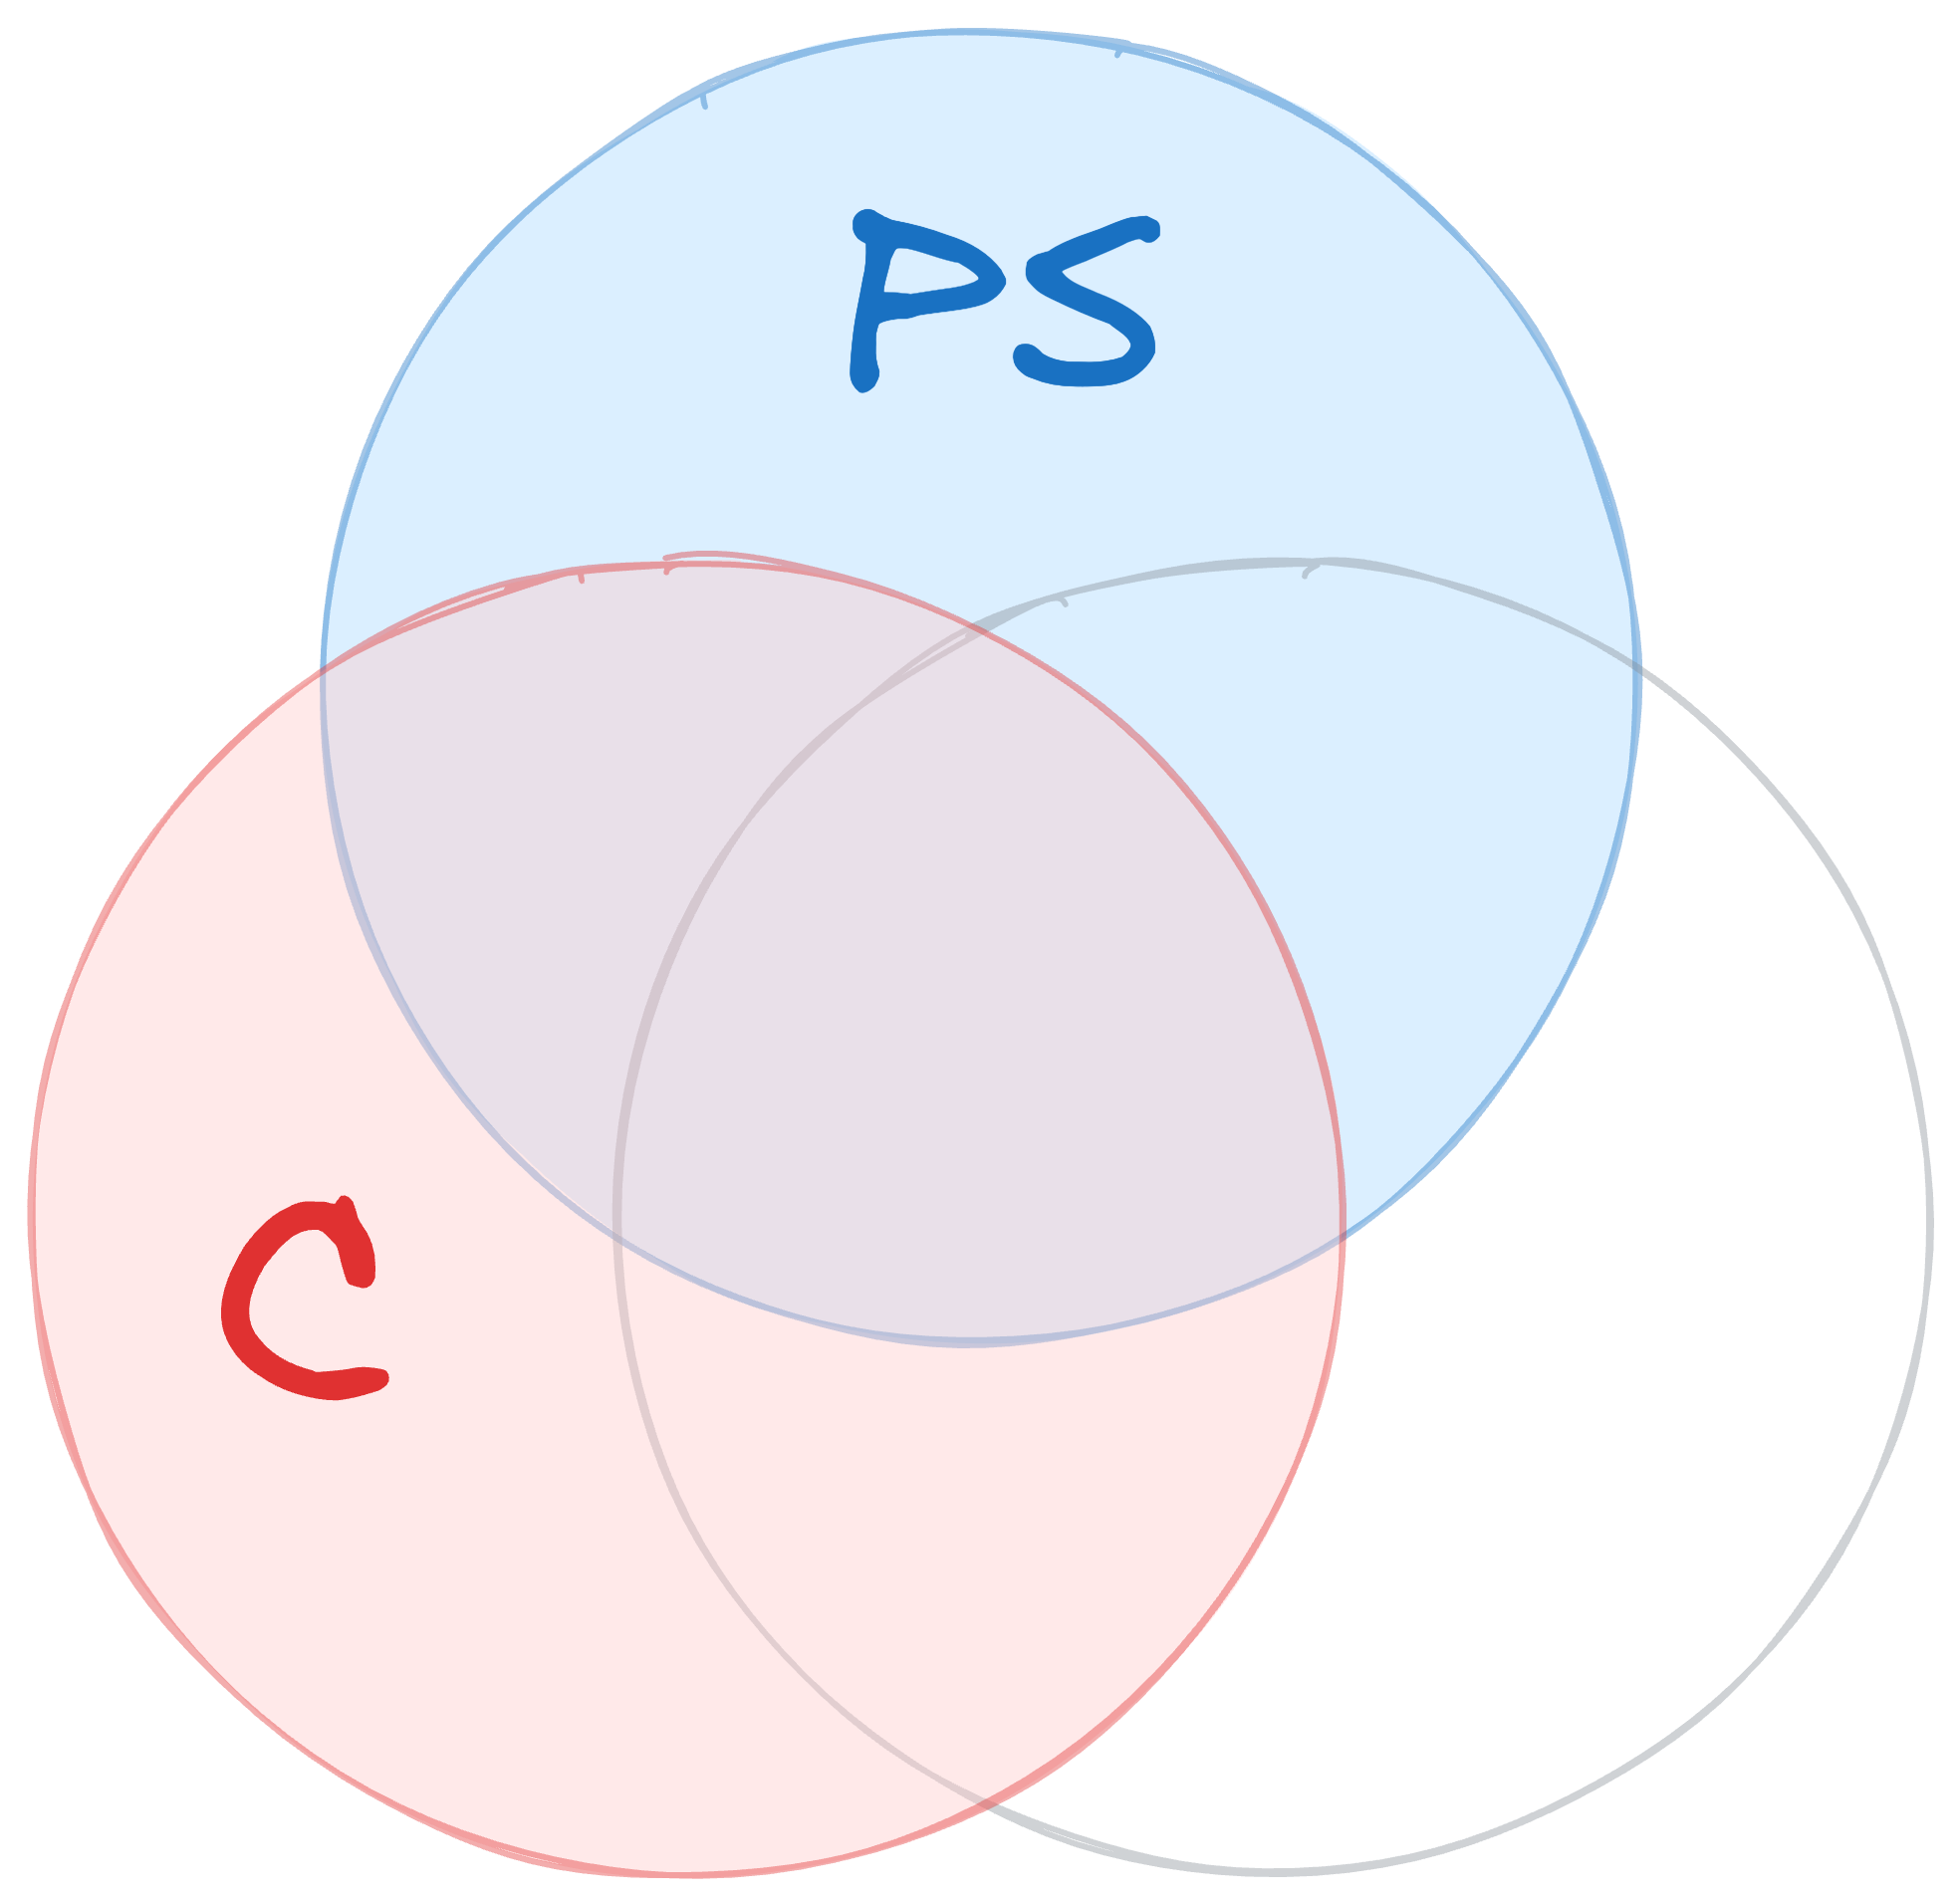
\includegraphics[width=\marginparwidth]{Figures/topics_ctrl_ps.png}
}
\label{sec:controlPartiallySpecified}

% Types of partial specification
The notion of \emph{partial specification} plays a central role in this thesis, and it appears in various forms within discrete system modeling. Broadly speaking, partial specification refers to situations in which some aspects of a system's structure or behavior are unknown, undefined, or only partially observable. This incompleteness poses a unique challenge for control, as it requires strategies that remain effective despite the inherent uncertainty. In the following paragraphs, we discuss several interpretations of partial specification and their relevance to Boolean network control.


% Non-observability
\emph{Non-observability} is considered to be one of the forms of the partial specification, since in such systems, the current state of the system cannot always be determined precisely~\cite{Kalman1960}. This challenge has long been recognized in control theory~\cite{Flokentin1962, Sorenson1968}, as we can not optimize control for the source state (because it is unknown). Non-observability is particularly common in biological systems where the full internal state is often hidden, or changing too rapidly to measure.~\cite{Liu2013,Villaverde2019} In the context of Boolean networks (BNs), we adopt a similar view: the internal dynamics are considered unobservable, and only attractors (i.e., stable, long-term behaviors) are assumed measurable. This abstraction is essential in biological modeling, where stable phenotypes correspond to observable steady states. Nonetheless, this thesis is concerned with an even broader and more complex notion of partial specification.


% Non-determinism
Another important source of uncertainty is \emph{non-determinism}, especially relevant in asynchronous BN. In such systems, the exact transition path from one state to another is not deterministic — multiple successor states may exist. This lack of transition determinsm can be viewed as a form of partial specification, as it obscures the system’s exact evolution over time. However, in this thesis, we treat non-determinism as an intrinsic property of the system rather than as an imperfection in its specification. The control task must therefore account for all possible transitions, ensuring control guarantee across all potential execution paths.


% Game theory, Mandon
Nondeterminism also inspired a game theoretic interpretation of control. In this perspective, the system and its uncertain evolution are viewed as an adversarial player, and the controller must identify a winning strategy to guide the system to a desired state~\cite{Mandon2019PHD}. This view is particularly useful in multistep control problems, where strategies unfold over multiple transitions and must remain effective despite adversarial behaviors. While the game theoretic approach provides valuable conceptual insight, the focus of this thesis lies in simpler control settings (e.g., single-step or permanent control), where the full strategy does not need to be explicitly constructed.


% Multiple possible functions 
A more structural form of partial specification arises in models such as \emph{probabilistic Boolean networks} (PBNs)~\cite{Shmulevich2002}, where uncertainty is introduced by allowing each variable to be governed by multiple update functions, each with an associated selection probability. In such models, not only is the update time of variables uncertain, but so is the logic guiding those updates. Thus, control must operate over a probability-weighted ensemble of behaviors, further complicating the synthesis of effective system perturbations.

In contrast, the \PBN{} framework central to this thesis allows each variable to have multiple possible update functions, but crucially assumes that only one “true” function per variable governs the evolution throughout the system's runtime. That is, while the identity of the function is unknown (and remains hidden due to nonobservability), it is assumed fixed. The resulting dynamics are therefore equivalent do asynchronous BN under a hidden function instance, though unknown from the observer’s perspective. This hybrid interpretation combines partial structural knowledge, non-determinism, and limited observability, creating a novel challenging control problem that this thesis aims to address.

% Partial functions?

% Control of other partially specified discrete systems?
% The control of partially specified systems is also closely related to the broader framework of discrete event systems (DES), where uncertainties arise in timing, event ordering, and transition logic. Similar challenges are present in stochastic models such as Markov chains and probabilistic transition systems. These models share structural affinities with PBNs, particularly in how transitions are defined over distributions rather than deterministic rules. These are a few examples which were inspiration for development of the BN. Now let's focus on the control of BN and methods closer to our approach. 



\section{Control of synchronous Boolean networks} 
\label{sec:controlSynchronous}
\marginpar{
    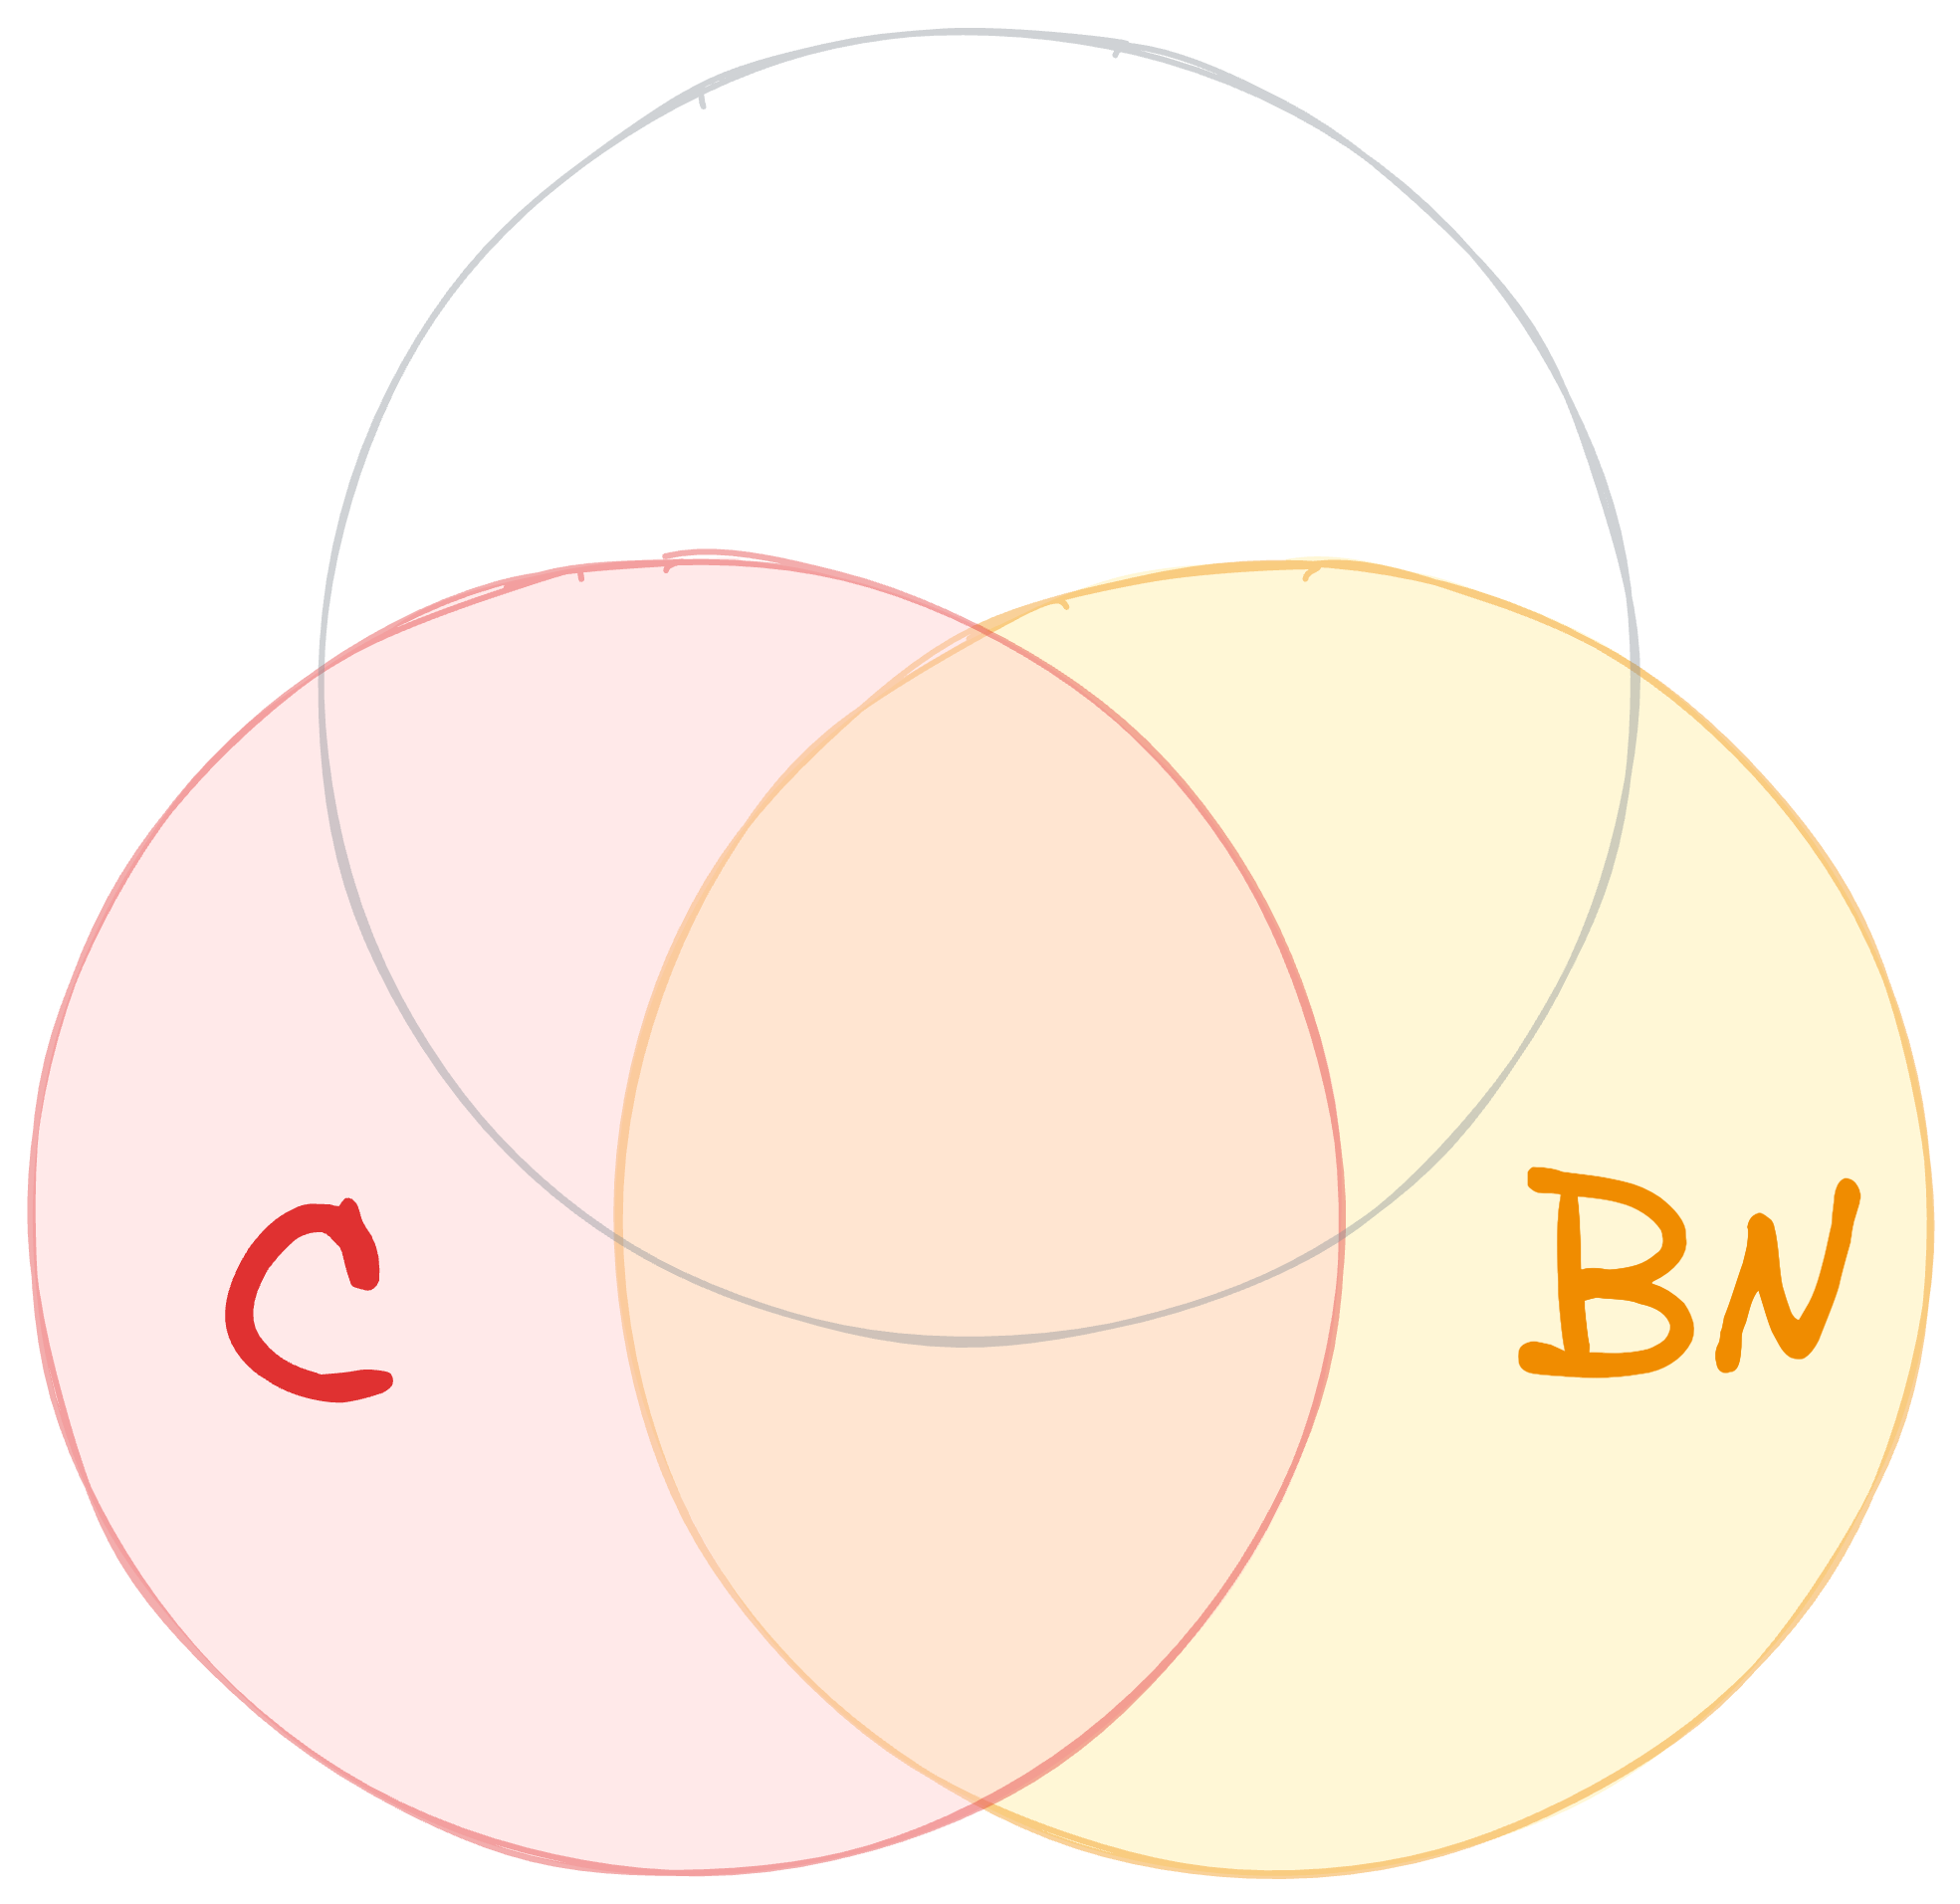
\includegraphics[width=\marginparwidth]{Figures/topics_ctrl_bn.png}
}
% Control of synchronous networks
Synchronous Boolean networks are characterized by the \emph{simultaneous} update of all variables at each time step. This deterministic update scheme ensures that the system's evolution is fully determined by its initial state. Despite this determinism, research on control for synchronous BNs remains highly relevant, especially because it provides foundational insights and inspiration for tackling more complex cases, such as asynchronous or partially specified networks.

% BCN relationship
As discussed earlier, control of Boolean control networks (BCNs) represents the most basic form of  BN control. In BCNs, control inputs can be modeled as direct perturbations of network variables or update rules. Therefore, if one enumerates all possible perturbations as  BN inputs and adjusts update functions accordingly, BCN-based control can trivially solve the control problem for synchronous BNs. Nonetheless, this naive approach is exponentially complex. Moreover, despite the deterministic underlying dynamics, the control problem for synchronous BN remains computationally challenging as it was proven to be NP-hard~\cite{Akutsu2007}.

% ASP
Given the Boolean nature of BN, an interesting problem reduction to the \emph{answer set programming} (ASP) was explored in~\cite{Kaminski2013}. The encoding of the problem here is quite straightforward, as the BN can be represented as a logic program, the control problem is formulated as a query, and even perturbations can be expressed as additional rules very conveniently by using three-valued logic. The approach was proven efficient, being handle to solve BN with up to 200 variables and perturbation size 10. A slightly generalized approach was later developed, allowing to specify general changes in long-term behavior (as opposed to output behavior only). Finally, ASP was also used to not just control the BN but also to infer input-output experiments and design therapeutic targets also packaged as a tool caspo~\cite{Videla2014,Videla2017}.

% One-step control
Beyond basic control problem, several more refined problem variations have emerged over time. Notably, Kim et al.~\cite{Kim2013} introduced the notion of a \emph{control kernel}, which is defined as the minimal set of variables that need to be set \emph{initially} in order to drive the system toward a desired attractor. This formulation corresponds to a one-step control problem and is closely aligned with the concept of perturbation strategies discussed in \autoref{subsec:perturbations}. 

% Phenotype control
Another perspective is provided by Choo et al.~\cite{Choo2018}, who generalized the target of control from a specific attractor to a broader \emph{phenotype}, defined as a set of target states sharing functional or biological characteristics. This abstraction reduces the granularity of control targets and allows for more flexible solution spaces. While computationally simpler than controlling asynchronous or partially specified networks, phenotype-based control provides valuable conceptual tools. Indeed, as discussed in \autoref{chapter:phenotype_control_psbn}, a similar generalization is central to our own contributions in control of \PBN{}.

% Ensembles control
A particularly relevant concept introduced for synchronous BNs is the control of \emph{Boolean network ensembles}~\cite{Gates2016,Correia2018,Gates2021,Videla2017}. In this setting, one considers a family of networks with identical topology but differing update functions. The control problem becomes finding a perturbation that guarantees convergence to the same attractor across all network instances. This notion aligns closely with the challenges posed by partial specification as we will see later in this work.

%Our own approach, presented in \autoref{chap:source_target_control}, generalizes this idea by relaxing the requirement for perturbations to strictly control every possible instance. This enables a framework for \emph{control-guided network inference}, as will be elaborated in \autoref{X}.

% Attractor computation
Finally, synchronous dynamics can also serve as a useful tool for analyzing asynchronous networks. Specifically, attractors identified under synchronous updates can act as approximations or partial indicators of stable attractors in the asynchronous setting~\cite{Zheng2013}. While this correspondence is limited to certain classes of attractors (e.g., stable fixed points), it provides valuable structural insights that can guide further analysis of asynchronous dynamics.


\section{Control of asynchronous Boolean networks} 
\label{sec:controlAsynchronous}

At the beginning of writing this thesis, the closest related work was the control of asynchronous BN~\cite{Smijakova2020}. Asynchronous BN offer a more biologically realistic modeling framework, as they incorporate asynchronous variable updates~\cite{Chaves2005}. This added expressiveness, however, introduces significant challenges for control, since the system's evolution is no longer deterministic and may follow multiple trajectories from the same initial state. To address this complexity, a broader variety control techniques were developed. In the following subsections, we survey key approaches to the control of asynchronous BN, highlighting the methods employed, the types of perturbations considered, and the formulation of control objectives.


\subsection{Refined strong basins search} \label{ss:strongbasinidentification}

Another branch of methods solving the BN control problem is based on the efficient identification of the strong basin of a target attractor (see \autoref{ss:state_space_structures}). By definition, a strong basin is the maximal set of states from which only the given attractor is reachable. Once the strong basin is identified, the control task reduces to finding the minimal perturbation that drives the BN into this basin. This is effectively a solution to the source-target control problem using one-step perturbations, since the solution there is as trivial as finding a state from strong basin with minimal Hamming distance to the source state. However, when considering other types of perturbations (e.g., temporary or permanent), additional computational steps are needed to determine appropriate control strategies.

A trivial approach to identifying the strong basin is through a fixed-point algorithm: nodes are iteratively removed from the weak basin if they have transitions that lead outside the basin. When no such nodes remain, the resulting set constitutes the strong basin. While conceptually simple, this method does not scale well for large biological networks. To address this limitation, a more efficient algorithm was proposed by Paul et al.~\cite{Paul2018BCB}, based on a decomposition of the state-transition graph (STG) into blocks.

The core idea of this block-based method is to partition the STG into basic blocks, where each block consists of a strongly connected component and its parent states. These blocks are considered in partial projections of the BN (subsets of the full variable set). Once identified, the blocks are topologically sorted and then unfolded, starting from the block containing the attractor, until all states in the strong basin are identified.

Compared to the stable motif approach that was discussed previously, strong basin identification must be performed separately for each target attractor when solving more complex variants of the control problem, such as full-control or all-pair control. Nonetheless, for smaller BN, the decomposition-based method has shown better performance even in full-control scenarios~\cite{Paul2018CMSB}, whereas for larger networks, the stable motif-based method tends to remain more efficient.

The strong basin identification approach has been successfully applied to source-target control with a variety of perturbation types: one-step initial perturbations~\cite{Paul2018BCB, Paul2018CMSB}, temporary and permanent perturbations~\cite{Su2019FM}, and sequential (attractor-based) variants~\cite{Mandon2019CMSB, Su2020}. More recently, the method has been extended to support target control under all types of perturbations~\cite{Su2020BCB,Su2020phd}. All of these techniques have been integrated into the software toolkit CABEAN~\cite{Su2020Bioinformatics}, facilitating broader adoption and experimentation.

\subsection{Stable motifs identification} \label{ss:stablemotifidentification}

Some techniques address complexity of asynchronous BN by analyzing only RN along with the update functions at first. The obtained information can be used to dramatically reduce the size of explicit state space, which needs to be explored to solve the BN control problem. 

One such approach is based on identification of \emph{stable motifs}~\cite{Zanudo2013,Zanudo2015}. A stable motif is a subset of variables and their corresponding values that, once reached, remain unchanged indefinitely. By identifying all stable motifs, one can construct a so-called \emph{succession diagram} that captures all possible nondeterministic runs of a BN. This diagram provides a structured way to navigate through the system's dynamics and determine the appropriate interventions needed to reach a desired attractor.

The strength of this method lies in its global topological analysis, which enables efficient performance. Once stable motifs are identified, they can be reused to compute control strategies for any attractor within the BN. This facilitates a solution to the full-control variant of the problem and offers valuable insights into the system robustness. However, the method is not complete as it may miss some viable control strategies. Additionally, stable motifs primarily serve as guidance for control design and must be validated through simulation to confirm their effectiveness. This validation also determines whether the required perturbations should be applied transiently (temporarily) or permanently.

To support broader adoption, the method was later implemented as a Python package, significantly improving its performance as well as accessibility for the research community~\cite{Rozum2022}.

\subsection{Trap spaces} 
\label{ss:asp}

Another approach based observing partially stabilized components is based on observing so-called \emph{value percolations}. This phenomenon is observed if we generalize successor function from a single state to subspaces. This way we can very quickly trace how the reachable subspaces from a given perturbation. Such an approach was first employed by aforementioned approach for the synchronous BN~\cite{Krumsiek2011,Videla2017}.

The downside of potential percolation-only approach for asyn\-chro\-nous BN is that it is not complete, since it does not guarantee to discover all perturbation strategies. Therefore, it was extended later by combining percolations with trap spaces exploration~\cite{Fontanals2020}. Trap spaces are spaces of the BN which can not be left once reached (see \autoref{ss:state_space_structures}). 

Compared to the strong basin, however, if we find a trap space in a \emph{synchronous} BN, the trap spaces are also contained in network's \emph{asynchronous} dynamics. Therefore, we can transfer the knowledge obtained from analysis of a simpler dynamics of synchronous BNs and use it for computing control of asynchronous BNs. The perturbations used in this approach are temporary state perturbations. 

Since the target of the method is a trap space, the target of the control is also generalized from a single attractor to an arbitrary subspace. This way the method is able to solve the control problem for a wider range of targets (attractors), and allow for more flexible control strategies. 

Given the nature of percolations and trapsaces, similar to the synchronous BN approach which inspired this work~\cite{Krumsiek2011}, methods for control of asynchronous BNs also use ASP to compute the control strategies. 

What is also interesting is that logical programming allowed to express the other types of perturbations than just variable perturbation, but also \emph{edge} perturbations, which disable a regulation of one variable to another~\cite{Fontanals2022c,Fontanals2023}.

It is worth mentioning, that there is also a significant body of work focusing solely on efficient computation of trap spaces. Therefore, tools and methods such as PyBoolNet~\cite{Klarner2018}, BioLQM~\cite{Naldi2018}, trappist~\cite{Trinh2022}, or tsconj~\cite{Trinh2024} can inspire future research of control methods.

\subsection{Model checking}
\label{ss:model_checking}

The methods based on percolation and trap spaces were limited to a specific subspace target (i.e., not a combination of multiple independent subspaces). Moreover, they needed to be combined with other approaches in order to obtain a complete solution to the control problem. These caveats inspired the development of a new method based on the model checking approach~\cite{Fontanals2022b}. 

The model-checking approach is using CTL to easily express the control problem. Nonetheless, the general model-checking approach tends to be slow since it explores the entire state space to make sure, that all states fulfill the properties.

Therefore, the control method itself is based on the idea of using a model checking as a ``backup'' approach if we are unable to assess whether a control strategy works using the trap-space-based method introduced previously. This way we obtain both, high performance for the majority of the cases and a complete solution for the rest.


\subsection{Other techniques}
Finally, we describe other techniques to control asynchronous BN which do not fit into the previous categories, because they use less conventional or a combination of multiple methods.

Kali is a tool for performing in silico therapeutic target discovery using network attractors~\cite{Poret2014,Poret2017,Poret2018}. The tool was in its last version updated to handle asynchronous and multivalued BNs. 

In this approach, the input is a physiological variant of the network and a pathological variant of the network. The goal is to find perturbations that drive the pathological variant to behave like the physiological one, i.e., to reach the same or at least a subset of the same attractors.

The approach is based on a combination of several techniques. First, the tool identifies all attractors of the BN using random walks. Then, so-called \emph{therapeutic bullets} candidates are generated, using uniform distribution of all possible options. These are combinations of ``bullet targets'' (states where perturbation is applied) and ``bullet values'' (the values to which the targets are perturbed).

The candidates are then evaluated by simulating the BN with applied bullet targets. The evaluation is based on the proportion of initial states reaching a physiological attractor or a portion of reachable physiological attractors in case of synchronous BN.

An interesting aspect of the method is, that not only universal perturbations are computed, but also \emph{existential} perturbations evaluated and quantified. Also, the method is focused on refining a model with the same behavior as opposed to driving it towards a specific static set of states. On the other hand, the method is not complete, since it relies on random walks to identify attractors and evaluate perturbations.

Another recently developed approach relies on semi-tensor products~\cite{Su2024}. This is another example of successful generalization of a technique working on synchronous BNs to asynchronous BNs. 
Again, given the nature of semi-tensor products, the control is achieved using periodical impulsive control. The viable controllers are defined along with the model, similarly to the synchronous BCNs mentioned in \autoref{sec:controlSynchronous}. 

Nonetheless, in this approach, the controllers do not need to be just static Boolean values, but can be also dynamic components that are gaining the value periodically. Moreover, this approach is able to quantify probability of reaching the target states as opposed to inevitably reach the state after applying the control.

\section{Control of most-permissive Boolean networks}
\label{sec:controlMostPermissive}

The previously described variants of BNs are limited in their ability to capture certain biologically significant behaviors~\cite{Pauleve2020}. For example, none of the earlier models can accurately represent the incoherent feed-forward loop of type 3 (I3-FFL)~\cite{Mangan2003}, a well-known motif in gene regulatory networks.

Most-permissive semantics enhances the expressiveness of BNs by allowing transient dynamics during state transitions from 0 to 1 and vice versa. This feature enables the representation of intermediate states, capturing subtleties in biological processes that are not strictly binary.

A major motivation for the development of most-permissive semantics lies in its application to model inference. The aim of model inference is to narrow down a broad set of candidate models to those that accurately reflect observed biological behavior. Under more restrictive Boolean semantics, correct models may be incorrectly discarded due to the absence of valid trajectories leading to experimentally observed attractors. As the name implies, most-permissive semantics allow the widest range of behaviors, thereby reducing the risk of false negatives during model selection.

An additional advantage of most-permissive Boolean networks is that despite their increased expressiveness they remain analytically tractable. In particular, Answer Set Programming (ASP) has proven to be well-suited for this framework, as it naturally supports the declarative encoding of Boolean logic and allows efficient searching for trajectories that either confirm or refute specific hypotheses~\cite{Pauleve2020}. However, a notable limitation of this approach is the difficulty in analyzing quantitative properties, such as the size of basins of attraction. For such purposes, simulation-based methods may be used, though they typically trade off completeness and performance~\cite{Roncalli2022}.

The tool BoNesis integrates various techniques for the analysis of most-permissive Boolean networks, including simulation, attractor detection, model synthesis, and control~\cite{Pauleve2023}. For symbolic reasoning it leverages ASP, enhanced with counterexample-guided abstraction refinement (CEGAR)~\cite{Riva2023}, while simulations of network dynamics are performed using an iterative depth-bounded approach.

Control within BoNesis is guided by specifying biological markers, which semantically correspond to the phenotypes introduced in \autoref{ss:model_checking}. The perturbations computed by the tool are permanent, and the control is universal, meaning that the desired properties must hold across all possible runs of the Boolean network. To minimize the size of the required perturbation set, users can optionally specify an initial configuration, thereby avoiding over-optimization across all possible initial states.

BoNesis supports differentiated control strategies for steady states (fixed points), and all attractors, enabling optimization tailored to task complexity, since reprogramming steady states is typically less computationally intensive~\cite{Pauleve2023}. Another notable feature of BoNesis is its ability to control ensembles of Boolean networks, which is especially relevant since model inference usually produces a set of plausible models rather than a single one. When controlling BN ensembles, users can choose between existential and universal control strategies. Existential control identifies perturbations that succeed in at least one model in the ensemble, while universal control yields perturbations that are guaranteed to work across all models.

\section{Leveraging control for model refinement}
\label{sec:controlInference}
\marginpar{
    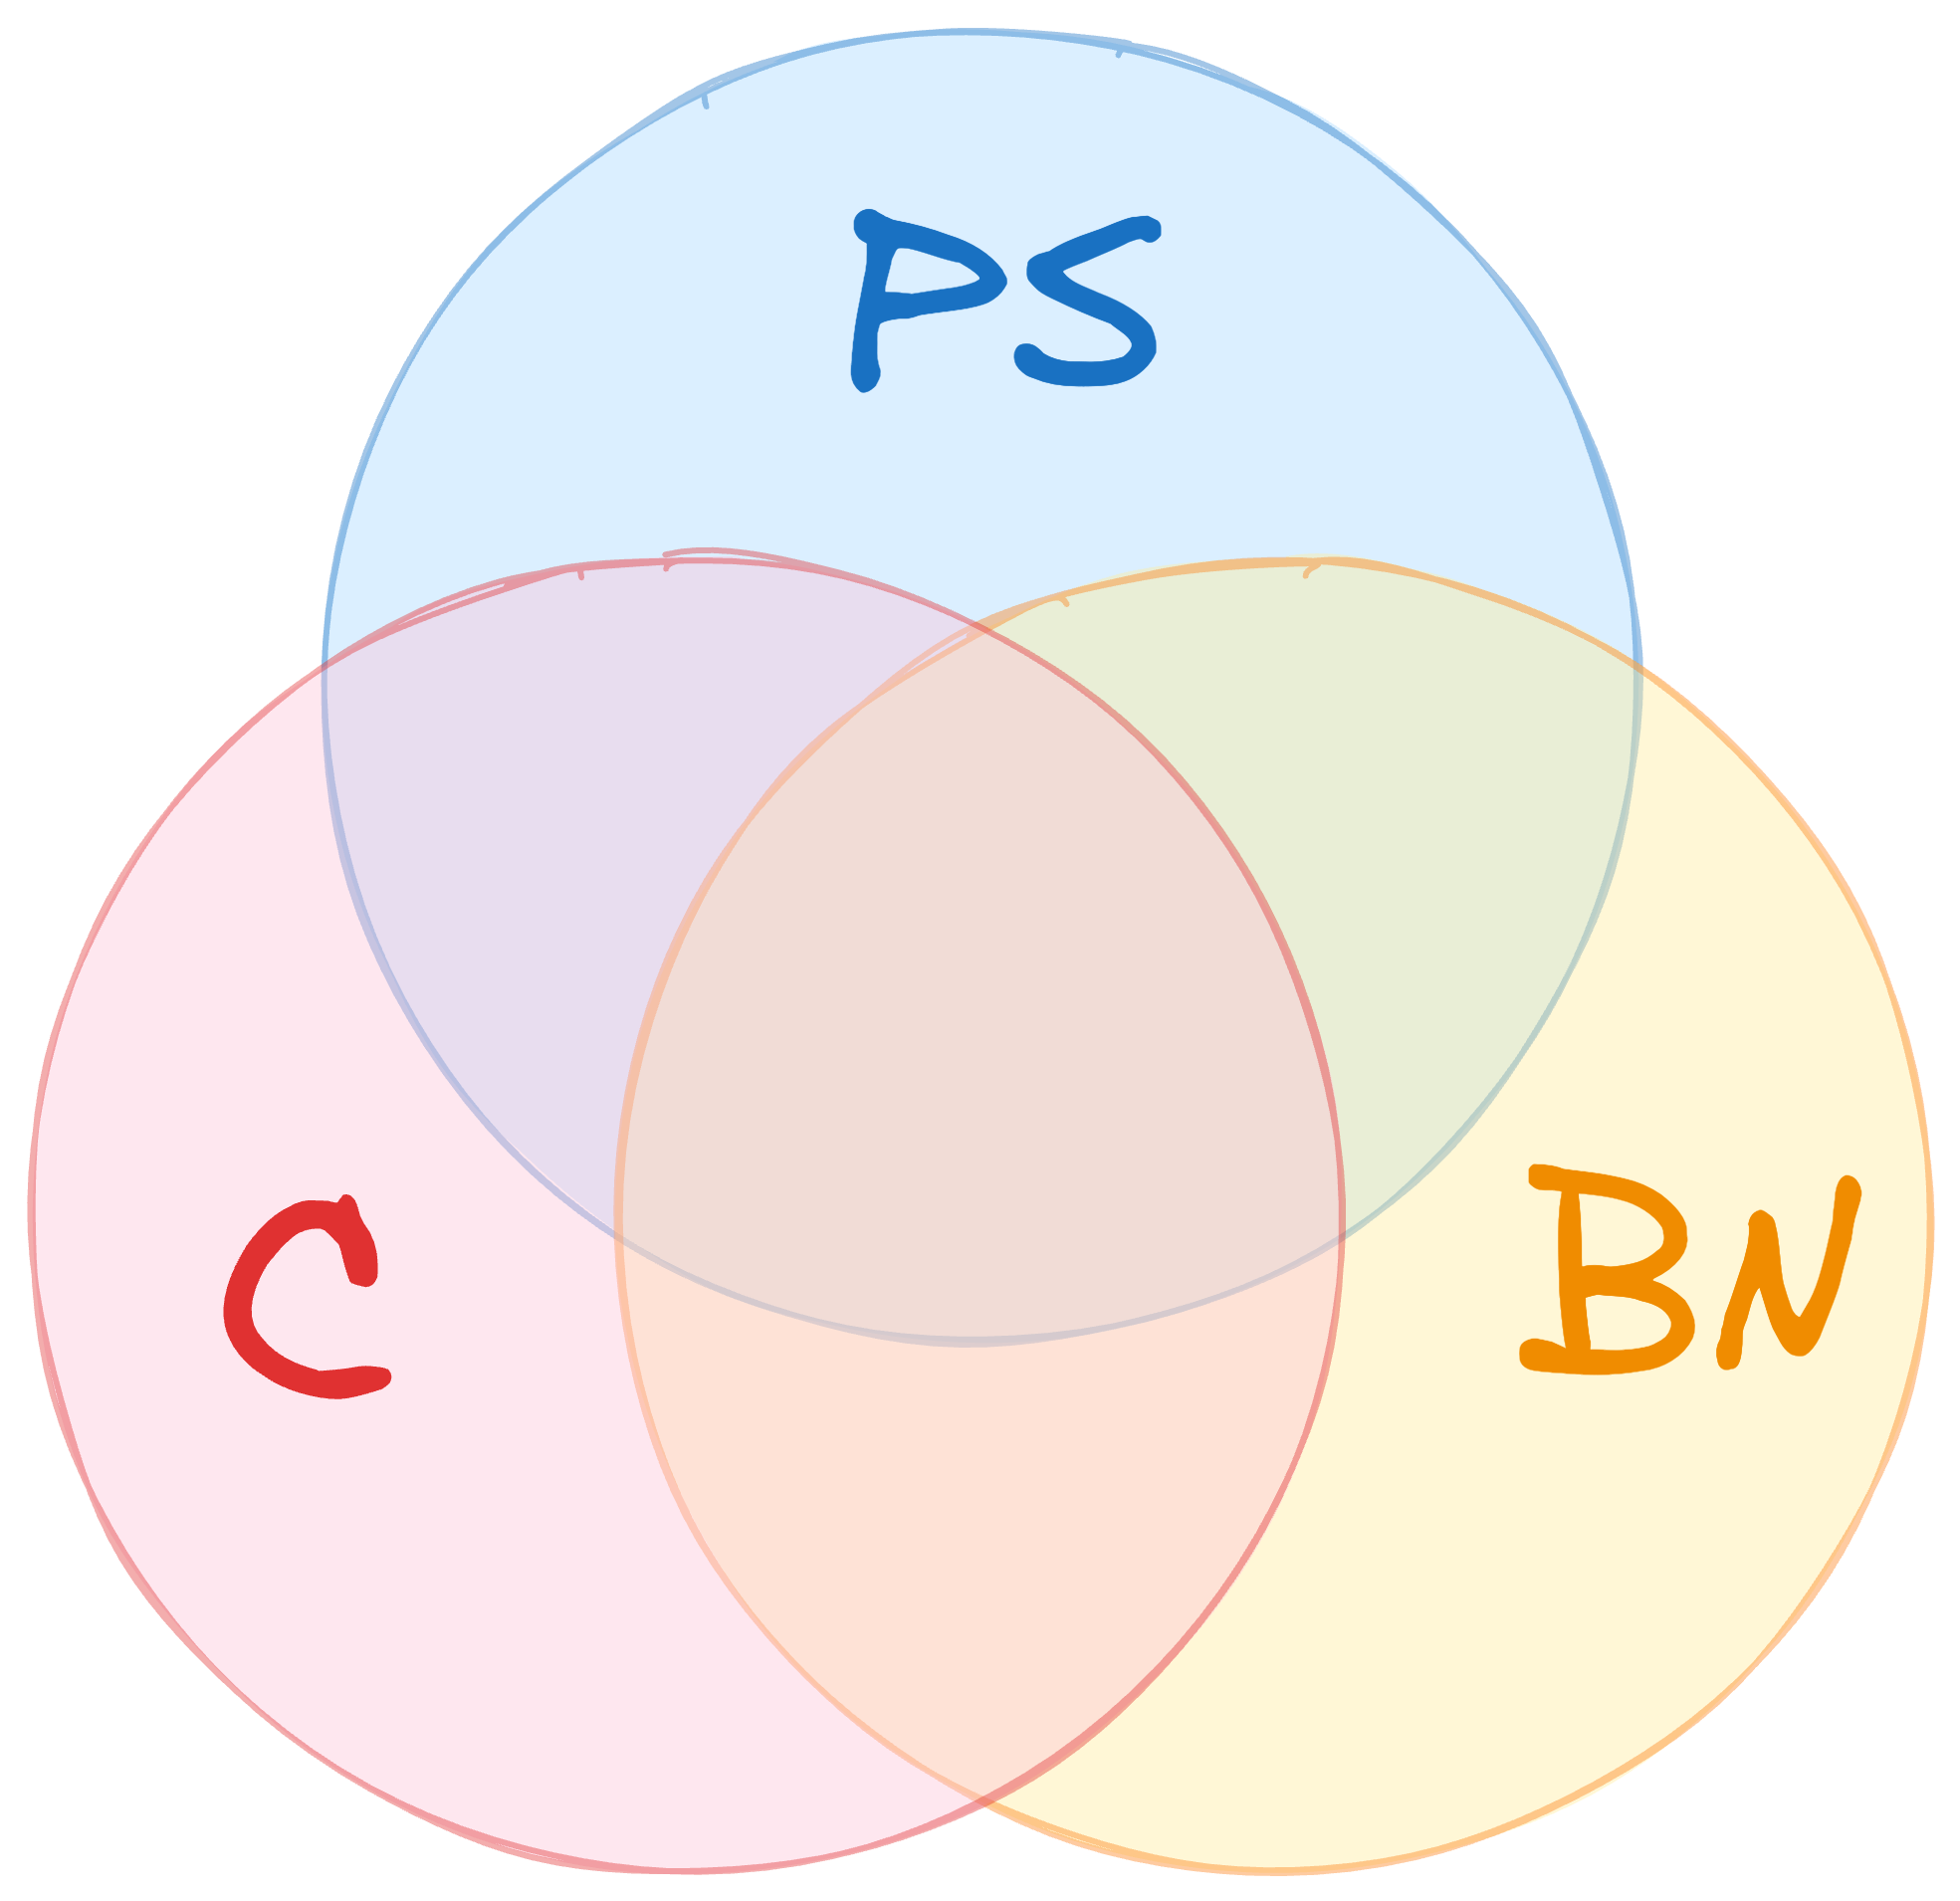
\includegraphics[width=\marginparwidth]{Figures/topics_all.png}
}

Traditionally, the control of Boolean networks has been viewed primarily as a means to modify system's  behavior, most notably for applications such as cellular reprogramming. However, recent research has begun to explore control as a valuable asset in the model refinement process. In this context, control can serve several important purposes:

\begin{enumerate}
    \item Handling uncertainty: Model inference may produce many network models that all fit the data. A good control strategy should work across these variations. If control leads all plausible models to the same desired behavior, it increases our confidence in both the models and the control itself~\cite{Chevalier2025}.
    \item Model verification: Control does not need to be just a downstream consumer of inferred models; it can also act as a verification tool. By applying perturbations and comparing the system's behavior to experimental observations, we can check that the model behaves in accordance with observations.
    \item Guiding experiments: When experimental data is limited or if there is an abundance of plausible models, control can help design better experiments. It can identify the most informative perturbations; those that produce system behaviors revealing how the network works.
\end{enumerate}

A growing body of work focuses on integrating perturbation data such as gene knockouts and over-expression experiments into the model inference pipeline~\cite{Gjerga2020,Yordanov2016,Park2025}. These efforts often rely on analyze model ensembles to explore the impact of perturbations. For instance, logic-based approaches can use Satisfiability Modulo Theories (SMT) to impose constraints on system dynamics, enabling the prediction of perturbation effects and facilitating model refinement based on experimental evidence~\cite{Yordanov2016}.

Control can also help prioritize new experiments by running in-silico simulations to predict which experiments would be most useful for refining the model. This idea originally came from continuous models, where system analysis has been used to design experiments that help fine-tune model parameters~\cite{Kreutz2009, Melykuti2010}. Later, similar strategies were applied to regulatory networks, where perturbation experiments were designed specifically to uncover the network's underlying structure~\cite{UdDean2016}.

Similar strategies have been developed for BNs, though with varying degrees of generality and scalability. Early works addressed experiment design for synchronous Boolean networks~\cite{Videla2015}. However, the only refined parts are inputs and outputs of the network, thus all available perturbations need to be included into model inputs beforehand.

Another line of work concerned with perturbations experiment design uses a maximum entropy framework to choose experiments that provide the most information~\cite{Atias2014}. Still, these methods rely heavily on simulations and are expected to be hard to scale; especially when dealing with asynchronous dynamics, where the number of possible system behaviors grows rapidly.


\section{Related tools}
\label{sec:relatedTools}

The majority of previously introduced methods were encompassed as software tools in order to make them accessible to a wider audience. Given the numerous nuances between control problems it is not an easy task to exhaustively compare the tools between them. Moreover, some features combinations might not be available. 

\begin{table}[]
    \label{tab:tools_compare}
    \centering
    \scalebox{0.8}{
    \begin{tabular}{rccccccl}
    \textbf{Tool} & \rot{\textbf{Source-targ.}} & \rot{\textbf{Target}} & \rot{\textbf{Phenotypes}} & \rot{\textbf{Partial spec.}} & \rot{\textbf{Pert. types}} & \rot{\textbf{Complete}} & \textbf{Main method} \\
    CABEAN  & ? & x & X & X & X & X & Strong basin search, ASP \\
    BoolNet & ? & x & X & X & X & X & X \\
    KALI    & ? & x & X & X & X & X & X \\
    CASPO   & ? & x & X & X & X & X & X \\
    BoNesis & ? & x & X & X & X & X & ASP \\
    AEON    & ? & x & X & X & X & X & BDDs, Symbolic 
    \end{tabular}
    }
    \caption{Comparison of related software tools for Boolean network control.}
\end{table}

\section{Summary}
\label{sec:sota_summary}


